\documentclass[
    ngerman,
    color=3b,
    % dark_mode,
    load_common, % Loads a list of commonly used Packages
    summary,
    boxarc,
    % manual_term,
    % solution=true,
]{tuda_summary} 
% Import all Packages from Main Preamble with relative Path
% \subimport*{../../}{preamble}
% Get Labels from Main Document using the xr-hyper Package
\externaldocument{../../AuD-Zusammenfassung-2020}
% Set Graphics Path, so pictures load correctly
\graphicspath{{../../}}


\begin{document}
\section{Grundlegende Datenstrukturen}\index{Grundlegende Datenstrukturen}
\subsection{Stacks}\label{Stacks}\index{Stacks}
\paragraph{Abstrakter Datentyp Stack}
\begin{description}[leftmargin=3cm,itemsep=1em]
    \item [\texttt{new S()}]
          \begin{itemize}
              \item Erzeugt neuen (leeren) Stack
          \end{itemize}
    \item [\texttt{s.isEmpty()}]
          \begin{itemize}
              \item Gibt an, ob Stack \texttt{s} leer ist
          \end{itemize}
    \item [\texttt{s.pop()}]
          \begin{itemize}
              \item Gibt oberstes Element vom Stack \texttt{s} zurück und löscht es vom Stack
              \item Gibt Fehlermeldung aus, falls der Stack leer ist
          \end{itemize}
    \item [\texttt{s.push(k)}]
          \begin{itemize}
              \item Schreibt \texttt{k} als neues oberstes Element auf Stack \texttt{s}
          \end{itemize}
\end{description}
\paragraph{Abstrakter Aufbau}\mbox{}
\fatsf{LIFO}-Prinzip - Last in, First out\index{LIFO}
\begin{figure}[ht]
    \centering
    \includestandalone[width=6cm]{pictures/LIFO/lifo}
    \caption{Abstrakter Aufbau eines Stacks}
    \label{fig:lifo}
\end{figure}


\paragraph{Beispiel Bitcoin}\index{Bitcoin}\mbox{}\\
\includestandalone[width=15cm]{pictures/bitcoin_stack_example/bitcoin_stack_example}
\clearpage
\paragraph{Stacks als Array}\mbox{}
\begin{figure}[ht]
    \centering
    \includestandalone[]{pictures/staack_als_array/stack_als_array}
    \caption{Beispiel: Stack als Array}
\end{figure}
\begin{description}[leftmargin=3cm,itemsep=1em]
    \item [\texttt{s.top}] zeigt immer auf oberstes Element
    \item [\texttt{pop()}] führt dazu, dass \texttt{s.Top} sich eins nach links bewegt
    \item [\texttt{push(k)}] führt dazu, dass \texttt{s.Top} sich eins nach rechts bewegt
\end{description}

\paragraph{Stacks als Array - Methoden, falls maximale Größe bekannt}\mbox{}\\
\begin{minipage}[t]{.5\textwidth}\mbox{}
    %\begin{noindent}
    \begin{codeBlock}[autogobble]{title=new(S)}
        S.A[]=ALLOCATE(MAX);
        S.top=-1;
    \end{codeBlock}
    %\end{noindent}
\end{minipage}
\begin{minipage}[t]{.5\textwidth}\mbox{}
    %\begin{noindent}
    \begin{codeBlock}[autogobble]{title=isEmpty(S)}
        IF S.top<0 THEN
          return true;
        ELSE
          return false;
    \end{codeBlock}
    %\end{noindent}
\end{minipage}
\begin{minipage}[t]{.5\textwidth}\mbox{}
    %\begin{noindent}
    \begin{codeBlock}[autogobble]{title=pop(S)}
        IF isEmpty(S) THEN
          error "underflow";
        ELSE
          s.top=s.top-1;
          return S.A[S.top+1];
    \end{codeBlock}
    %\end{noindent}
\end{minipage}
\begin{minipage}[t]{.5\textwidth}\mbox{}
    %\begin{noindent}
    \begin{codeBlock}[autogobble]{title=push(S)}
        IF S.top==MAX-1 THEN
          error "overflow";
        ELSE
          S.top=S.top+1;
          S.A[S.top]=k;
    \end{codeBlock}
    %\end{noindent}
\end{minipage}
%\item[] 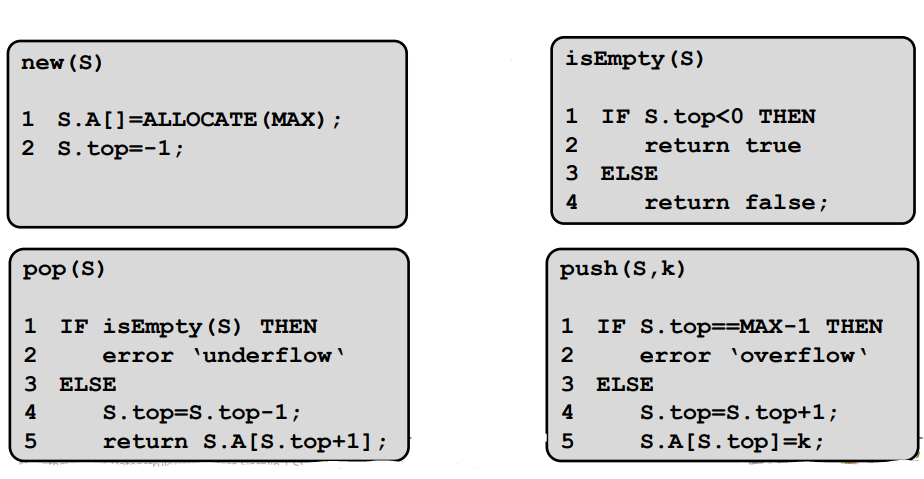
\includegraphics[width=12cm]{pictures/arrayMethods1}

\paragraph{Stacks mit variabler Größe - Einfach}
\begin{itemize}
    \item Falls \texttt{push(k)} bei vollem Array $\Rightarrow$ Vergößerung des Arrays
    \item Erzeugen eines neuen Arrays mit Länge + 1 und Umkopieren aller Elemente
    \item Durchschnittlich $\Omega(n)$ Kopierschritte pro \texttt{push}-Befehl
\end{itemize}
\clearpage
\paragraph{Stacks mit variabler Größe - Verbesserung}\mbox{}
\begin{idea}[Stacks mit Variabler Größe]\mbox{}
    \begin{itemize}
        \item Wenn Grenze erreicht, Verdopplung des Speichers und Kopieren der Elemente
        \item Falls weniger als ein Viertel belegt, schrumpfe das Array wieder
    \end{itemize}
\end{idea}
Methoden:
\texttt{RESIZE(A,m)} reserviert neuen Speicher der Grö\ss e \texttt{m} und kopiert \texttt{A} um\\
\begin{minipage}[t]{.5\textwidth}\mbox{}
    %\begin{noindent}
    \begin{codeBlock}[autogobble]{title=new(S)}
        S.A[]=ALLOCATE(1);
        S.top=-1;
        S.memsize=1;
    \end{codeBlock}
    %\end{noindent}
\end{minipage}
\begin{minipage}[t]{.5\textwidth}\mbox{}
    %\begin{noindent}
    \begin{codeBlock}[autogobble]{title=isEmpty(S)}
        IF S.top<0 THEN
            return true;
        ELSE
            return false;
    \end{codeBlock}
    %\end{noindent}
\end{minipage}
\begin{minipage}[t]{.5\textwidth}\mbox{}
    %\begin{noindent}
    \begin{codeBlock}[autogobble]{title=pop(S)}
        IF isEmpty(S) THEN
            error "underflow";
        ELSE
            S.top=S.top-1;
            IF 4*(S.top+1)==S.memsize THEN
                S.mensize=s.memsize/2;
                RESIZE(S.A,S.memsize);
            return S.A[S.top+1];
    \end{codeBlock}
    %\end{noindent}
\end{minipage}
\begin{minipage}[t]{.5\textwidth}\mbox{}
    %\begin{noindent}
    \begin{codeBlock}[autogobble]{title=push(S)}
        S.top=S.top+1;
        S.A[S.top]=k;
        IF S.top+1>=S.memsize THEN
            S.memsize=2*S.memsize;
            RESIZE(S.A,S.memsize);
    \end{codeBlock}
    %\end{noindent}
\end{minipage}
%\item[] 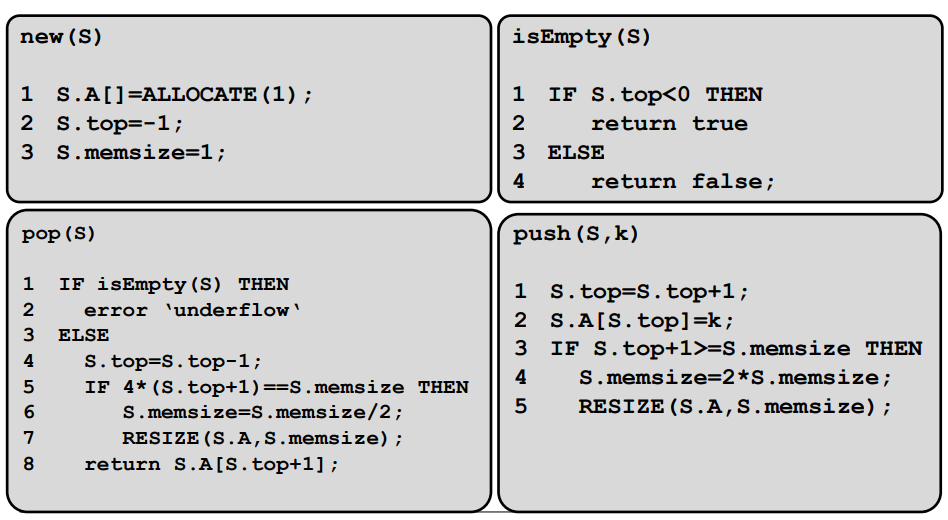
\includegraphics[width=12cm]{pictures/stacksArray2.PNG}

Im Durchschnitt für jeder der mindestens \texttt{n} Befehle $\Theta(1)$ Umkopierschritte


\clearpage
\subsection{Verkettete Listen}\label{Verkettete Listen}\index{Verkettete Listen}
\paragraph{Aufbau}\mbox{}
\begin{figure}[h]
    \centering
    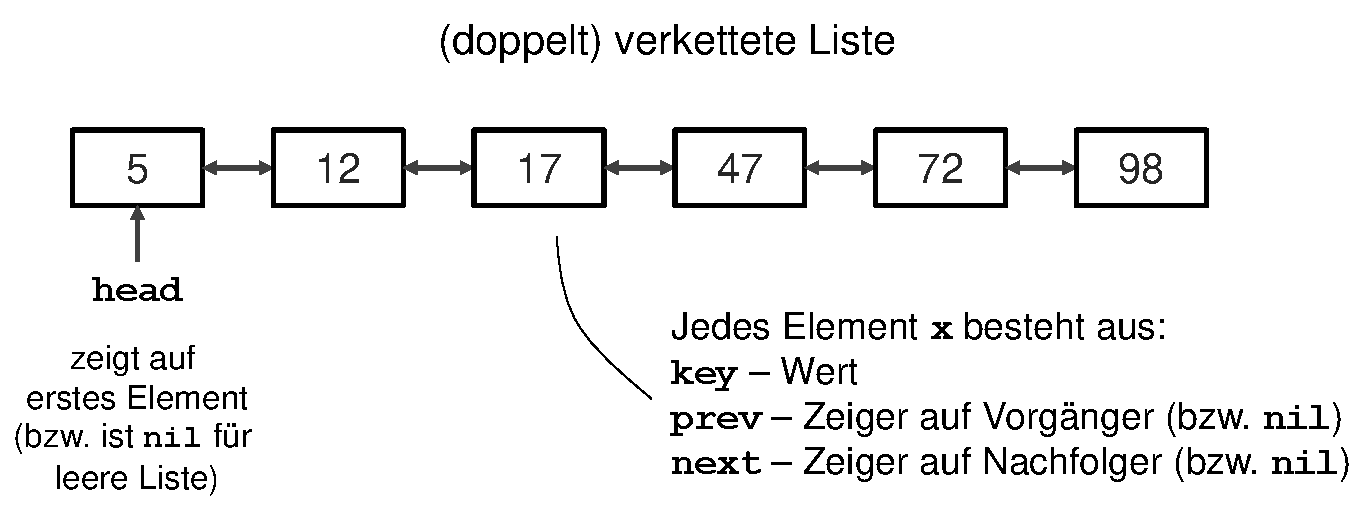
\includegraphics[width=12cm]{pictures/linkedList1.pdf}
    \caption{Aufbau Verkettete Liste}
\end{figure}


\paragraph{Verkettete Listen durch Arrays}\mbox{}\\
Entspricht doppelter Verkettung zwischen 45 und 12
\begin{figure}[h]
    \centering
    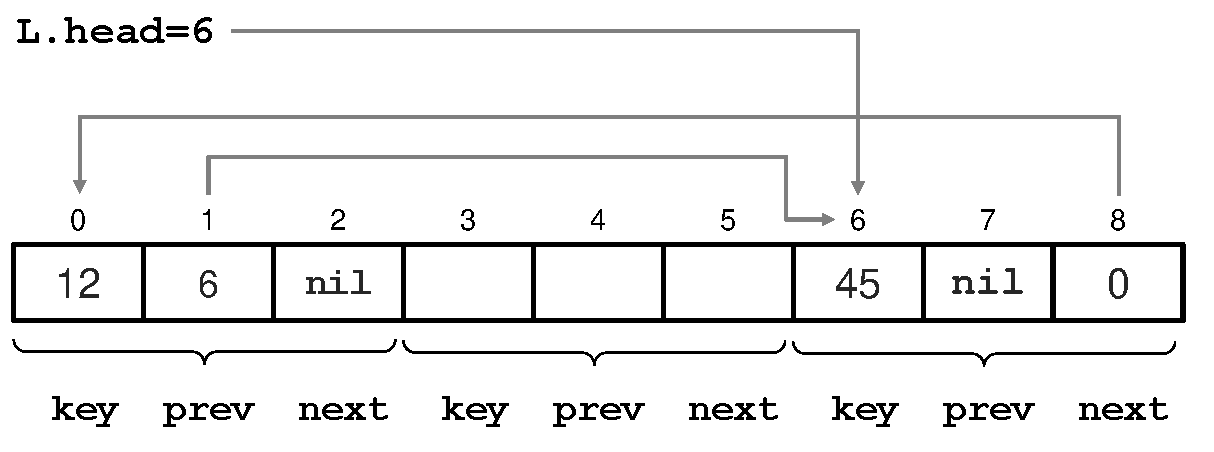
\includegraphics[width=12cm]{pictures/linkedList2.pdf}
    \caption{Beispiel Verkettete Liste durch Arrays}
\end{figure}

\clearpage
\subsubsection{Elementare Operationen auf Listen}
\paragraph{Suche nach Element}\mbox{}
%\begin{noindent}
\begin{codeBlock}[autogobble]{title={search(L,k) // Returns pointer to k in L (or nil)}}
    current = L.head;
    WHILE current != nil AND current.key != k DO
      current = current.next;
    return current;
\end{codeBlock}
%\end{noindent}
Laufzeit beträgt im Worst Case $\Theta(n)\Rightarrow$ Keine Überprüfung, ob Wert bereits in Liste, sonst $\Theta(n)$
\begin{figure}[h]
    \centering
    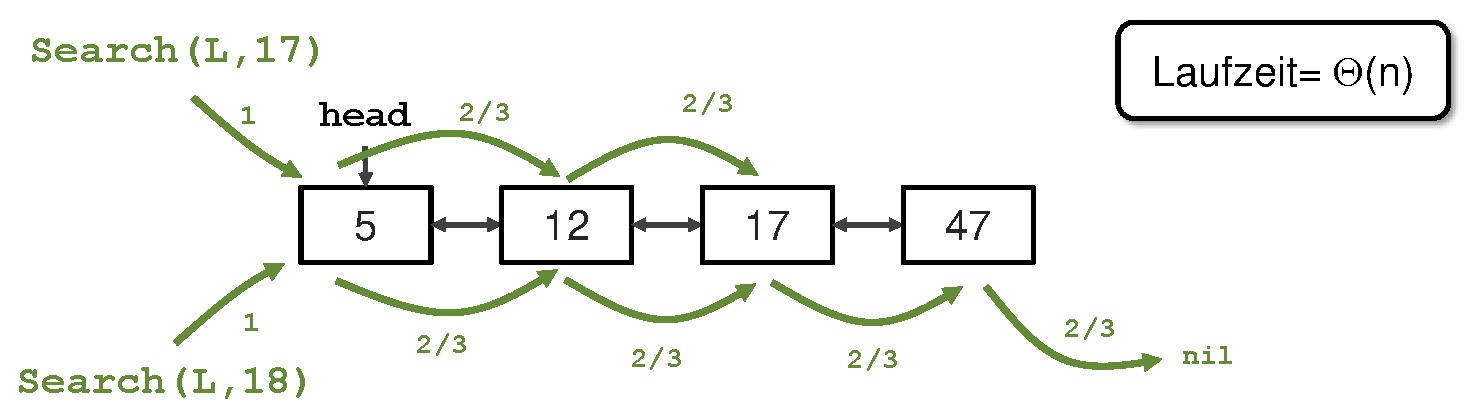
\includegraphics[width=12cm]{pictures/verketteteListenSuche.pdf}
    \caption{Grafische Darstellung einer Suche in Listen}
\end{figure}
\FloatBarrier
\vspace{-1cm}
\begin{minipage}[t]{.49\textwidth}\mbox{}
    \paragraph{Einfügen eines Elements am Kopf der Liste}\mbox{}
    %\begin{noindent}
        \begin{codeBlock}[autogobble]{title={insert(L,x)}}
            insert(L,x)
            x.next = l.head;
            x.prev = nil;
            IF L.head != nil THEN
                L.head.prev = x;
            L.head = x;
        \end{codeBlock}
        %\end{noindent}
    Laufzeit beträgt $\Theta(1)$, da Einfügen am Kopf
\end{minipage}
\begin{minipage}[t]{.5\textwidth}\mbox{}
    \paragraph{Löschen eines Elements aus Liste}\mbox{}
    %\begin{noindent}
    \begin{codeBlock}[autogobble]{title={delete (L,x)}}
        IF x.prev != nil THEN
          x.prev.next = x.next
        ELSE
          L.head = x.next;
        IF x.next != nil THEN
          x.next.prev = x.prev;
    \end{codeBlock}
    %\end{noindent}
    Laufzeit beträgt $\Theta(1)$, da hier Pointer auf Objekt gegeben
    Löschen eines Wertes $k$ mithilfe von Suche beträgt $\Omega(n)$
\end{minipage}

\paragraph{Vereinfachung per Wächter/Sentinels}\index{Sentinel}\mbox{}\\
Ziel ist die Eliminierung der Spezialfälle für Listenanfang/-ende
\begin{figure}[h]
    \centering
    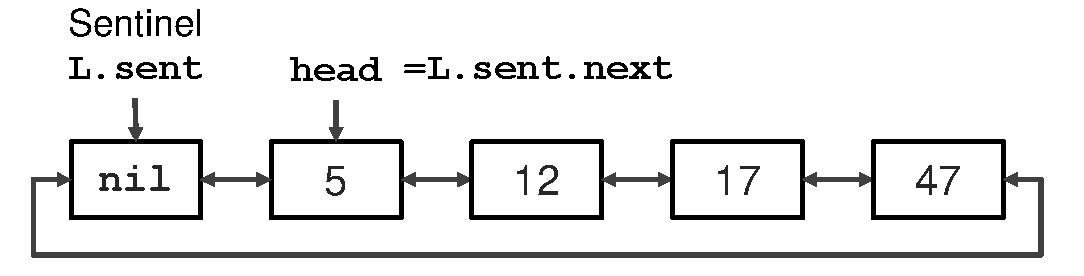
\includegraphics[width=10cm]{pictures/linkedListSentinel.pdf}
    \caption{Beispiel Sentinel}
\end{figure}\mbox{}\\
Löschen mit Sentinels:
%
%\begin{noindent}
\begin{codeBlock}[autogobble]{title={deleteSent(L,x)}}
    x.prev.next = x.next;
    x.next.prev = x.prev;
\end{codeBlock}
%\end{noindent}
\clearpage
\subsection{Queues}\label{Queues}\index{Queue}
\paragraph{Abstrakter Datentyp Queue}
\begin{description}[leftmargin=3cm,itemsep=1em]
    \item [\texttt{new Q()}]
          \begin{itemize}
              \item Erzeuge neue (leere) Queue
          \end{itemize}

    \item [\texttt{q.isEmpty()}]
          \begin{itemize}
              \item Gibt an, ob Queue \texttt{q} leer ist
          \end{itemize}

    \item [\texttt{q.dequeue()}]
          \begin{itemize}
              \item Gibt vorderstes Element aus \texttt{q} zurück und löscht es auf Queue
              \item Fehlermeldung, falls Queue leer ist
          \end{itemize}

    \item [\texttt{q.enqueue(k)}]
          \begin{itemize}
              \item Schreibt \texttt{k} als neues hinterstes Element auf \texttt{q}
              \item Fehlermeldung, falls Queue voll ist
          \end{itemize}

\end{description}

\paragraph{Abstrakter Aufbau}\mbox{}\\
\fatsf{FIFO}-Prinzip\index{FIFO} / First in, First out
\begin{figure}[h]
    \centering
    \includestandalone[width=8cm]{pictures/FIFO/FIFO}
    \caption{Beispiel FIFO}
\end{figure}
\clearpage

\paragraph{Queues als (virtuelles) zyklisches Array}\index{zyklisches Array}\mbox{}\\
Bekannt: Maximale Elemente gleichzeitig in Queue
\begin{figure}[ht]
    \centering
    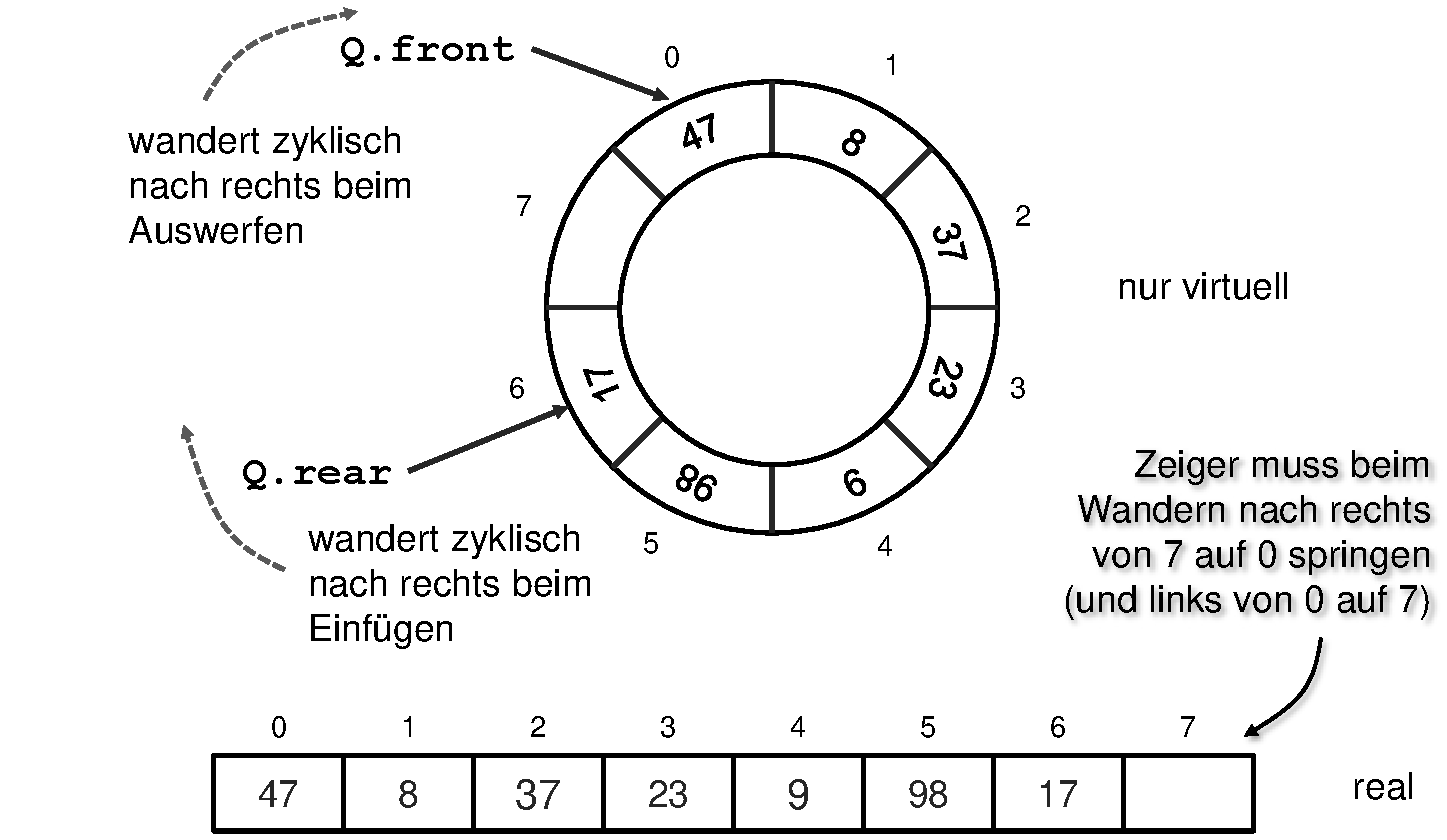
\includegraphics[width=12cm]{pictures/queueZyklisch.pdf}
    \caption{Beispiel Queue als Zyklisches Array}
\end{figure}

Problem, falls \texttt{Q.rear} und \texttt{Q.front} auf selbes Element zeigen
\begin{itemize}
    \item Speichere Information, ob Schlange leer oder voll, in boolean \texttt{empty}
    \item Alternativ: Reserviere ein Element des Arrays als Abstandshalter
\end{itemize}

Methoden für zyklisches Array:\\
\begin{minipage}[t]{.49\textwidth}\mbox{}
    %\begin{noindent}
    \begin{codeBlock}[autogobble]{title={new(Q)}}
        Q.A[]=ALLOCATE(MAX);
        Q.front=0;
        Q.rear=0;
        Q.empty=true;
    \end{codeBlock}
    %\end{noindent}
\end{minipage}
\begin{minipage}[t]{.5\textwidth}\mbox{}
    %\begin{noindent}
    \begin{codeBlock}[autogobble]{title={isEmpty(Q)}}
        return Q.empty;
    \end{codeBlock}
    %\end{noindent}
\end{minipage}

\begin{minipage}[t]{.49\textwidth}\mbox{}
    %\begin{noindent}
    \begin{codeBlock}[autogobble]{title={dequeue(Q)}}
        IF isEmpty(Q) THEN
            error "underflow";
        ELSE
            Q.front=Q.front+1 mod MAX;
            IF Q.front==Q.rear THEN
                Q.empty=true;
            return Q.A[Q.front-1 mod MAX];
    \end{codeBlock}
    %\end{noindent}
\end{minipage}
\begin{minipage}[t]{.5\textwidth}\mbox{}
    %\begin{noindent}
    \begin{codeBlock}[autogobble]{title={enqueue(Q,k)}}
        IF Q.rear==Q.front AND !Q.isEmpty
        THEN error "overflow";
        ELSE
            Q.A[Q.rear]=k;
            Q.rear=Q.rear+1 mod MAX;
            Q.empty=false;
    \end{codeBlock}
    %\end{noindent}
\end{minipage}
%\item[] 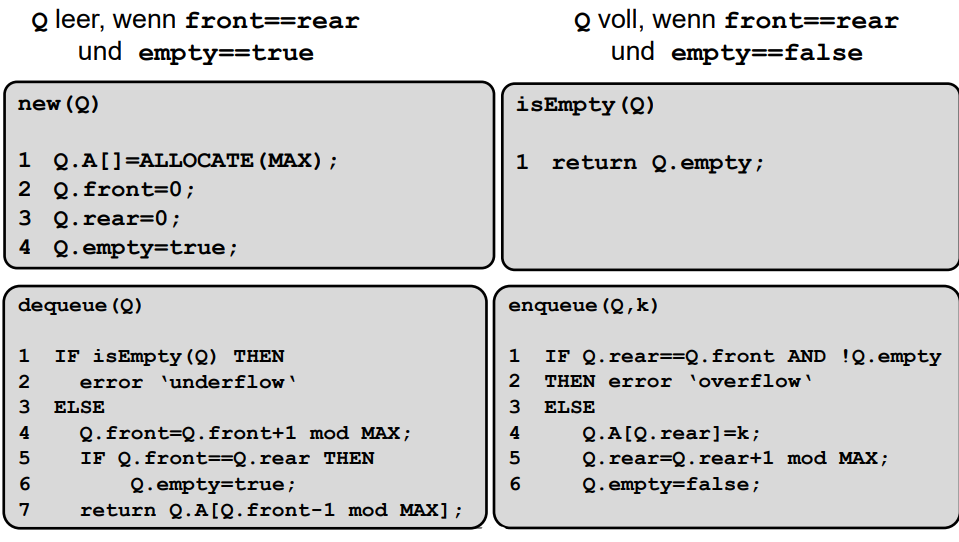
\includegraphics[width=12cm]{pictures/queueZyklischM.PNG}

\clearpage

\paragraph{Queues durch einfach verkettete Listen}\mbox{}
\begin{figure}[h]
    \centering
    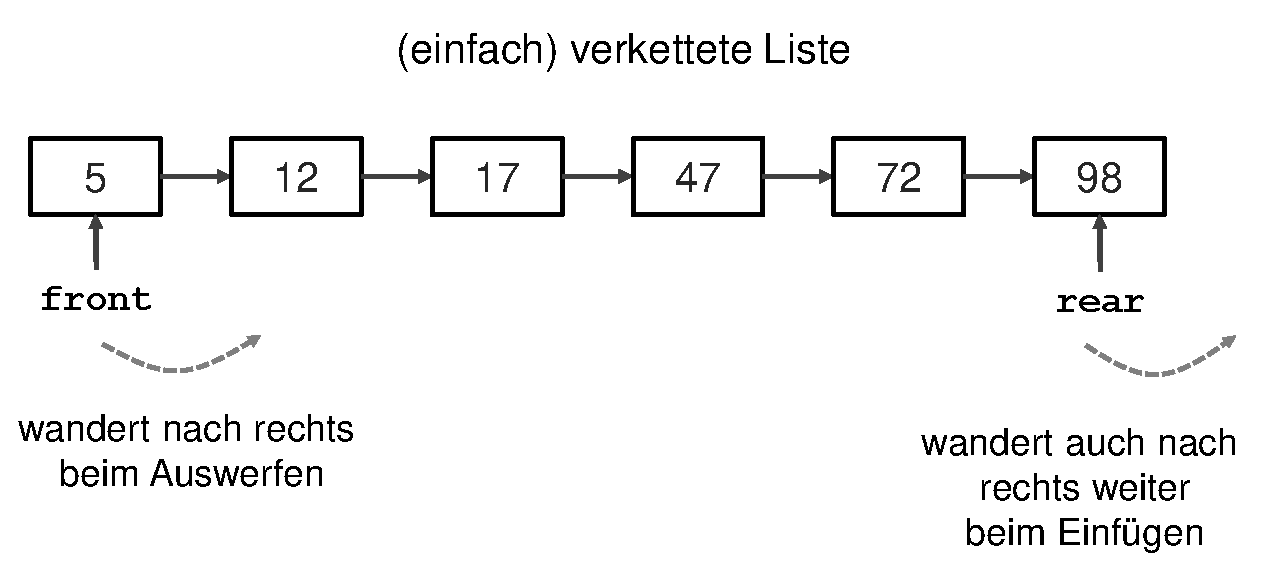
\includegraphics[width=12cm]{pictures/queuesListe1.pdf}
    \caption{Beispiel Queue durch einfach verkettete Liste}
\end{figure}
\FloatBarrier
Methoden:\\
%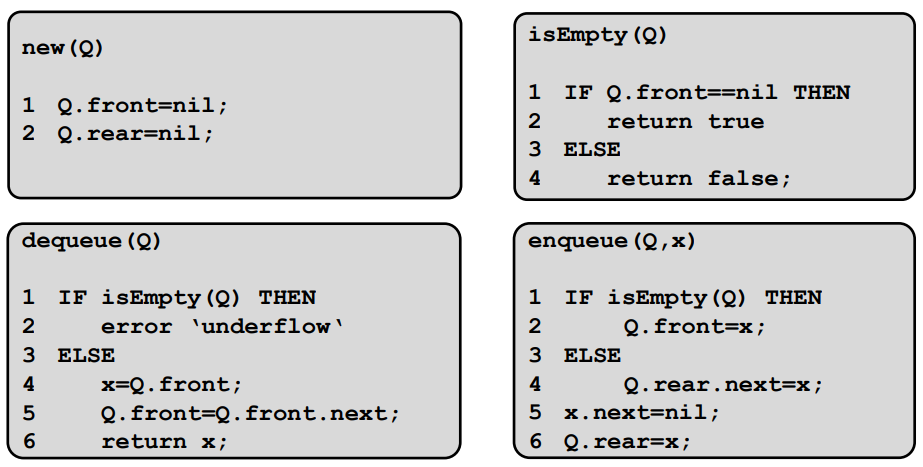
\includegraphics[width=12cm]{pictures/queuesListe2.PNG} 
\begin{minipage}[t]{.49\textwidth}\mbox{}
    %\begin{noindent}
    \begin{codeBlock}[autogobble]{title={new(Q)}}
        Q.front=nil;
        Q.rear=nil;
    \end{codeBlock}
    %\end{noindent}
\end{minipage}
\begin{minipage}[t]{.5\textwidth}\mbox{}
    %\begin{noindent}
    \begin{codeBlock}[autogobble]{title={isEmpty(Q)}}
        IF Q.front==nil THEN
            return true;
        ELSE
            return false;
    \end{codeBlock}
    %\end{noindent}
\end{minipage}
\\
\begin{minipage}[t]{.49\textwidth}\mbox{}
    %\begin{noindent}
    \begin{codeBlock}[autogobble]{title={dequeue(Q)}}
        IF isEmpty(Q) THEN
            error "underflow";
        ELSE
            x=Q.front;
            Q.front=Q.front.next;
            return x;
    \end{codeBlock}
    %\end{noindent}
\end{minipage}
\begin{minipage}[t]{.5\textwidth}\mbox{}
    %\begin{noindent}
    \begin{codeBlock}[autogobble]{title={enqueue(Q,k)}}
        IF isEmpty(Q) THEN
            Q.front=x;
        ELSE
            Q.rear.next=x;
        x.next=nil;
        Q.rear=x;
    \end{codeBlock}
    %\end{noindent}
\end{minipage}


Laufzeit:
\begin{itemize}
    \item Enqueue: $\Theta(1)$
    \item Dequeue: $\Theta(1)$
\end{itemize}

\clearpage
\subsection{Binäre Bäume}\label{Binaere Baeume}\index{Binäre Bäume}
\paragraph{Bäume durch verkettete Listen}\mbox{}
\begin{figure}[h]
    \centering
    \includegraphics[width=12cm]{pictures/binäreBaumeListe.PNG}
    \caption{Binärbaum-Beispiel}
\end{figure}
\FloatBarrier
Bäume sind \enquote{azyklisch}(also \enquote{keine Schleifen zwischen Knoten})

\paragraph{Darstellung als (ungerichteter) Graph}\mbox{}\\
\begin{minipage}[c]{0.49\textwidth}\mbox{}
    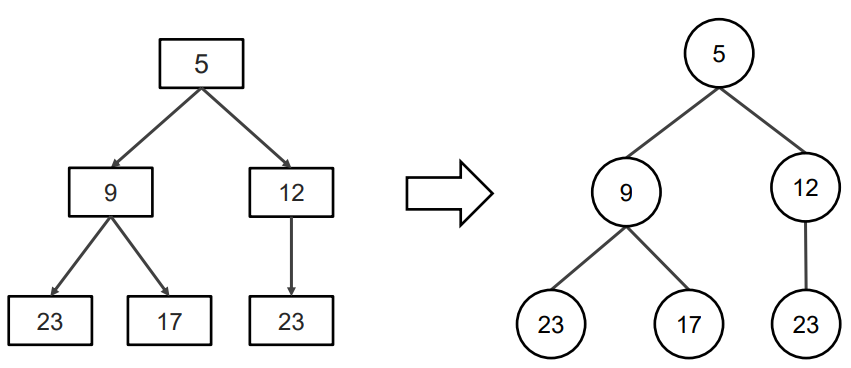
\includegraphics[width=\linewidth-5pt]{pictures/baumGraph1.PNG}
\end{minipage}
\begin{minipage}[c]{0.5\textwidth}\mbox{}
    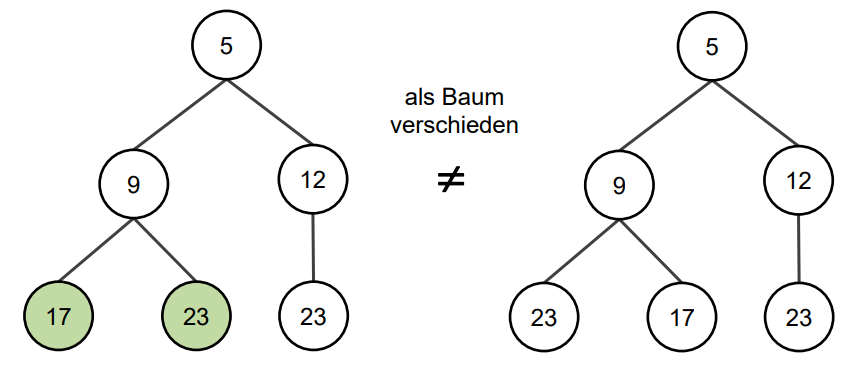
\includegraphics[width=\linewidth-5pt]{pictures/baumGraph2.PNG}
\end{minipage}

\paragraph{Allgemeine Begrifflichkeiten}\index{Vorfahre}\index{ancestor}\index{Wurzel}\index{root}\index{parent}\index{Elternknoten}\index{Kindknoten}\index{child}\index{Geschwisterknoten}\index{sibling}\index{Nachkomme}\index{descendant}\index{Blatt}\index{leaf}\index{Höhe (Baum)}\mbox{}\\

\begin{minipage}[c]{0.59\textwidth}\mbox{}
    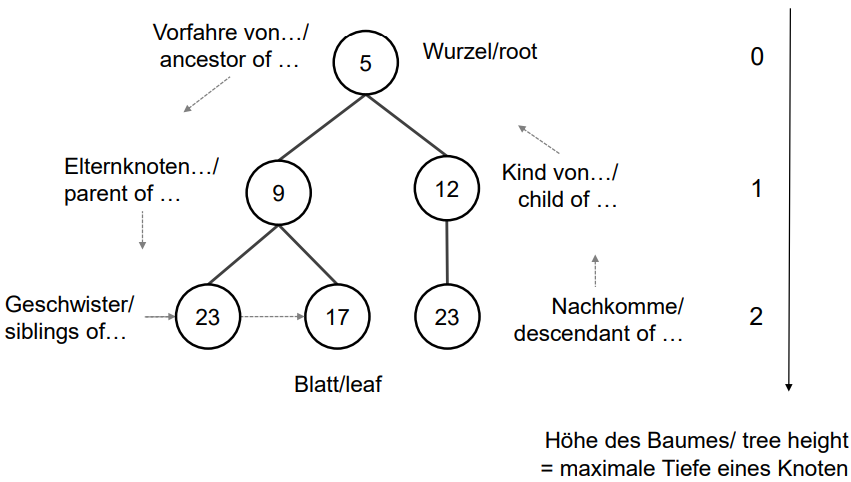
\includegraphics[width=\linewidth-10pt]{pictures/baumBegriffe1.PNG}
\end{minipage}
\begin{minipage}[c]{0.4\textwidth}\mbox{}
    \vspace{-.5cm}
    \begin{itemize}
        \item Blatt: Knoten ohne Nachfolger
        \item Nachkomme von x: \\
              Erreichbar durch Pfad ausgehend von x
    \end{itemize}
\end{minipage}

\clearpage
\paragraph{Begrifflichkeiten Binärbaum}\index{Halbblatt}\index{Teilbaum}\mbox{}\\
\begin{minipage}[c]{0.45\textwidth}\mbox{}
    \includegraphics[width=8cm]{pictures/binärbaumBegriffe}
\end{minipage}
\begin{minipage}[c]{0.45\textwidth}\mbox{}
    \begin{itemize}
        \item Jeder Knoten hat maximal zwei Kinder \\
              \texttt{left=child[0]} und \texttt{right=child[1]}
        \item Ausgangsgrad jedes Knoten ist $\leq 2$
        \item Höhe leerer Baum per Konvention $-1$
        \item Hohe (nicht-leerer) Baum: \\
              max\{Höhe aller Teilbäume der Wurzel\} + 1
        \item Halbblatt: Knoten mit nur einem Kind
    \end{itemize}
\end{minipage}



\paragraph{Traversieren von Bäumen}\index{Traversieren von Bäumen}
\begin{itemize}
    \item Darstellung eines Baumes mithilfe einer Liste der Werte aller Knoten
    \item Laufzeit bei $n$ Knoten: $T(n) = O(n)$
    \item Nutzung der Preorder für das Kopieren von Bäumen
          \begin{enumerate}
              \item Preorder betrachtet Knoten und legt Kopie an
              \item Preorder geht dann in Teilbäume und kopiert diese
          \end{enumerate}
    \item Nutzung der Postorder für das Löschen von Bäumen
          \begin{enumerate}
              \item Postorder geht zuerst in Teilbäume und löscht diese
              \item Betrachten des Knoten erst danach und dann Löschung dieses
          \end{enumerate}
\end{itemize}
\begin{minipage}[c]{0.4\textwidth}\mbox{}
    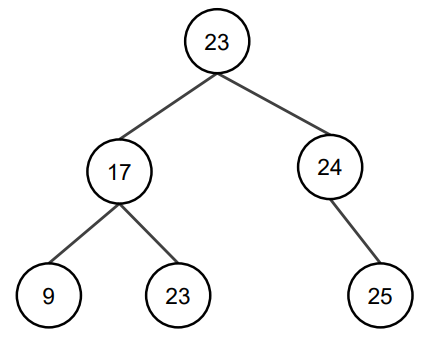
\includegraphics[width=6cm]{pictures/inorder1}
\end{minipage}
\begin{minipage}[c]{0.5\textwidth}\mbox{}
    \begin{itemize}
        \item[] 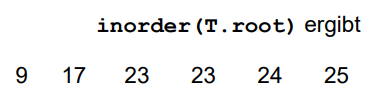
\includegraphics[width=6cm]{pictures/inorder2}
        \item[] 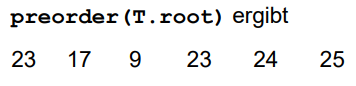
\includegraphics[width=6cm]{pictures/preorder1}
        \item[] 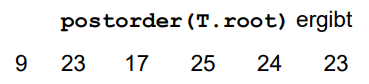
\includegraphics[width=6cm]{pictures/postorder1}
    \end{itemize}
\end{minipage}
\paragraph{Code:}\index{inorder}\index{preorder}\index{postorder}\mbox{}\vspace*{-1em}\\
\begin{minipage}[t]{0.33\linewidth}\mbox{}
    %\begin{noindent}
    \begin{codeBlock}[autogobble,fontsize=\small]{title={inorder(x)}}
        IF x != nil THEN
            inorder(x.left);
            print x.key;
            inorder(x.right);
    \end{codeBlock}
    %\end{noindent}
\end{minipage}
\begin{minipage}[t]{0.33\linewidth}\mbox{}
    %\begin{noindent}
    \begin{codeBlock}[autogobble,fontsize=\small]{title={preorder(x)}}
        IF x != nil THEN
            print x.key;
            preorder(x.left);
            preorder(x.right);
    \end{codeBlock}
    %\end{noindent}
\end{minipage}
\begin{minipage}[t]{0.33\linewidth}\mbox{}
    %\begin{noindent}
    \begin{codeBlock}[autogobble,fontsize=\small]{title={postorder(x)}}
        IF x != nil THEN
            postorder(x.left);
            postorder(x.right);
            print x.key;
    \end{codeBlock}
    %\end{noindent}
\end{minipage}
\clearpage
\paragraph{Eindeutige Bestimmbarkeit von Bäumen}
\begin{itemize}
    \item Nur In-, Pre-, Postorder reichen nicht zur eindeutigen Bestimmbarkeit von Bäumen
    \item[] $\Rightarrow$ Preorder/Postorder $+$ Inorder $+$ eindeutige Werte sind notwendig
    \item[] 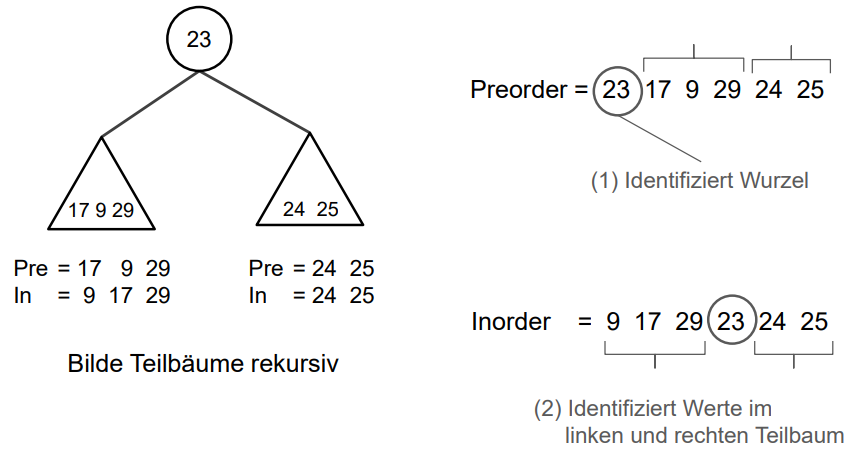
\includegraphics[width=12cm]{pictures/bestimmbarkeitBaum.PNG}
\end{itemize}


\subsubsection{Abstrakter Datentyp Baum}
\paragraph{Abstrakter Aufbau:}\mbox{}
\begin{description}[leftmargin=3cm,itemsep=.8em]
    \item [\texttt{new T()}]
          \begin{itemize}
              \item Erzeugt neuen Baum namens \texttt{t}
          \end{itemize}

    \item [\texttt{t.search(k)}]
          \begin{itemize}
              \item Gibt Element \texttt{x} in Baum \texttt{t} mit \texttt{x.key == k} zurück
          \end{itemize}

    \item [\texttt{t.insert(k)}]
          \begin{itemize}
              \item Fügt Element \texttt{x} in Baum \texttt{t} hinzu
          \end{itemize}

    \item [\texttt{t.delete(x)}]
          \begin{itemize}
              \item Löscht \texttt{x} aus Baum \texttt{t}
          \end{itemize}
\end{description}

\paragraph{Suche nach Elementen}

Starte mit \texttt{search(T.root,k)}
Code:

%\begin{noindent}
\begin{codeBlock}[autogobble]{title={search(x,k)}}
    IF x == nil THEN return nil;
    IF x.key == k THEN return x;
    y = search(x.left,k);
    IF y != nil THEN return y;
    return search(x.right,k);
\end{codeBlock}
%\end{noindent}
Laufzeit = $\Theta(n)$ (Jeder Knoten maximal einmal, jeder Knoten im schlechtesten Fall)
\clearpage
\paragraph{Einfügen von Elementen}\mbox{}\\
Hier wird als Wurzel eingefügt (Achtung: Erzeugt linkslastigen Baum)
Code:

%\begin{noindent}
\begin{codeBlock}[autogobble]{title={insert(T,x) // x.parent == x.left == x.right == nil;}}
    IF T.root != nil THEN
      T.root.parent = x;
      x.left = T.root;
    T.root = x;
\end{codeBlock}
%\end{noindent}
Laufzeit = $\Theta(1)$

\paragraph{Löschen von Elementen}\mbox{}\\
Hier: Ersetze $x$ durch Halbblatt ganz rechts
\begin{figure}[h]
    \centering
    \includegraphics[width=12cm]{pictures/löschenBaum.PNG}
    \caption{Löschen des Knoten 17}
\end{figure}
\clearpage
\texttt{Connect}-Algorithmus:\\
\begin{minipage}[c]{0.6\textwidth-1.853pt}
    %\begin{noindent}
    \begin{codeBlock}[autogobble]{title={connect(T,y,w) // Connects w to y.parent}}
        v = y.parent;
        IF y != T.root THEN
            IF y == v.right THEN
                v.right = w;
            ELSE
                v.left = w;
        ELSE
            T.root = w;
        IF w != nil THEN
            w.parent = v;
    \end{codeBlock}
    %\end{noindent}
    Laufzeit = $\Theta(1)$
\end{minipage}
\begin{minipage}[c]{0.4\textwidth}
    \centering
    \includegraphics[width=5cm]{pictures/löschenBaumConnect.PNG}
    \captionof{figure}{Beispiel Connect-Algorithmus Binärbaum}
\end{minipage}


\texttt{Delete}-Algorithmus:\\
\begin{minipage}{0.6\textwidth-1.853pt}

    %\begin{noindent}
    \begin{codeBlock}[autogobble]{title={delete(T,x) // assumes x in T}}
        y = T.root;
        WHILE y.right != nil DO
            y = y.right;
        connect(T,y,y.left);
        IF x != y THEN
            y.left = x.left;
            IF x.left != nil THEN
                x.left.parent = y;
            y.right = x.right;
            IF x.right != nil THEN
                x.right.parent = y;
            connect(T,x,y);
    \end{codeBlock}
    %\end{noindent}
    Laufzeit = $\Theta(h)$ (Höhe des Baumes, $h=n$ möglich)
\end{minipage}
\begin{minipage}{0.4\textwidth}
    \centering
    \includegraphics[width=6cm]{pictures/löschenBaumDelete.PNG}
    \captionof{figure}{Beispiel Delete-Algorithmus Binärbaum}
\end{minipage}


\clearpage
\subsection{Binäre Suchbäume}\label{Binaere Suchbaeume}\index{Binäre Suchbäume}
\begin{definition}[Binärer Suchbaum]
    \item Totale Ordnung auf den Werten
    \item Für alle Knoten $z$ gilt:
    \item[] Wenn $x$ Knoten im linken Teilbaum von $z$, dann \texttt{x.key $\leq$ z.key}
    \item[] Wenn $y$ Knoten im rechten Teilbaum von $z$, dann \texttt{y.key $\geq$ z.key}
    \item Preorder/Postorder + eindeutige Werte $\Rightarrow$ Eindeutige Identifizierung
\end{definition}

\paragraph{Suchen im Binären Suchbaum}\mbox{}\\


\begin{minipage}[c]{0.5\textwidth-1.85301pt}


    Code:
    %\begin{noindent}
    \begin{codeBlock}[autogobble]{title={search(x,k) // 1. Aufruf: x = root}}
        IF x == nil OR x.key == k THEN
          return x;
        IF x.key > k THEN
          return search(x.left,k);
        ELSE
          return search(x.right,k);
    \end{codeBlock}
    %\end{noindent}
    Iterativer Code:
    %\begin{noindent}
    \begin{codeBlock}[autogobble]{title={iterative-search(x,k)}}
        WHILE x != nil AND x.key != k DO
          IF x.key > k THEN
              x = x.left;
          ELSE
              x = x.right;
        return x;
    \end{codeBlock}
    %\end{noindent}
    Laufzeit (beide) $= O(h)$ (Höhe)
\end{minipage}
\begin{minipage}[c]{0.5\textwidth}
    \centering
    \includegraphics[width=9cm]{pictures/binärerSuchbaumSuche.PNG}
    \captionof{figure}{Beispiel Search-Algorithmus im Binärbaum}
\end{minipage}
\clearpage
\paragraph{Einfügen im Binary Search Tree}\mbox{}\\
Aufwendiger, da Ordnung erhalten werden muss
Code:\label{BST-Insert}
%\begin{noindent}
\begin{codeBlock}[autogobble]{title={insert (T,z) // z.left == z.right == nil;}}
    x = T.root;
    px = nil;
    WHILE x != nil DO
      px = x;
      IF x.key > z.key THEN
          x = x.left;
      ELSE
          x = x.right;
    z.parent = px;
    IF px == nil THEN
      T.root = z;
    ELSE
      IF px.key > z.key THEN
          px.left = z;
      ELSE
          px.right = z;
\end{codeBlock}
%\end{noindent}
Laufzeit = $O(h)$
\begin{figure}[h]
    \centering
    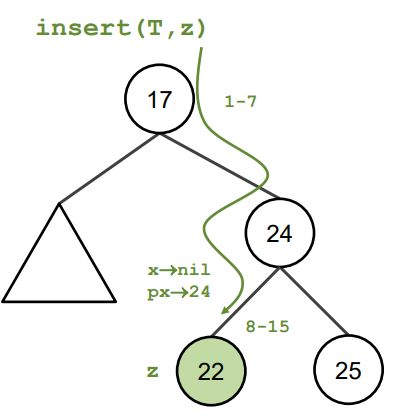
\includegraphics[width=8cm]{pictures/binärerSuchbaumEinfügen.PNG}
    \caption{Beispiel einfügen in Binären Suchbaum}
\end{figure}

\clearpage

\paragraph{Löschen im BST}\mbox{}\\
wir Unterscheiden drei verschiedene Fälle:
\begin{figure}[h]
    % \centering
    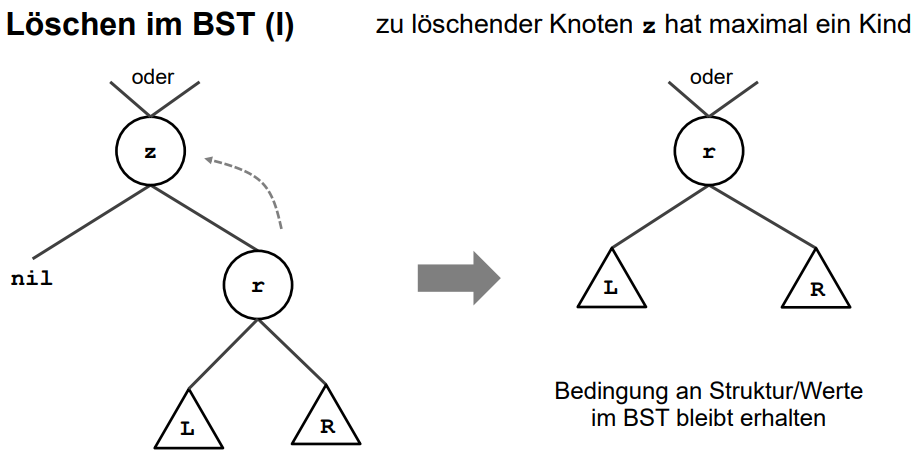
\includegraphics[width=9cm]{pictures/binärerSuchbaumLöschen1.PNG}
    % \caption{Löschen im BST-Fall 1}
\end{figure}
\begin{figure}[h]
    % \centering
    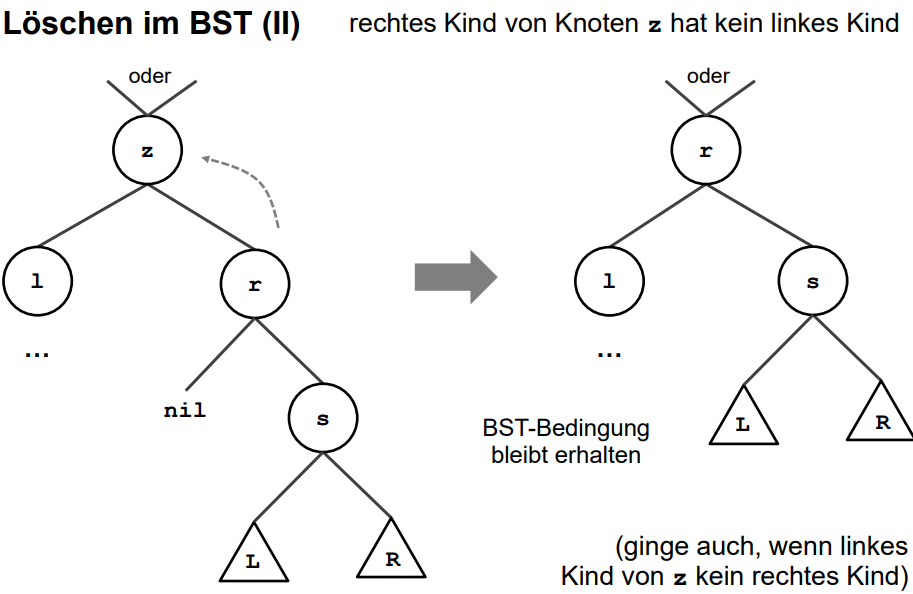
\includegraphics[width=9cm]{pictures/binärerSuchbaumLöschen2.PNG}
    % \caption{Löschen im BST-Fall 2}
\end{figure}
\begin{figure}[h]
    % \centering
    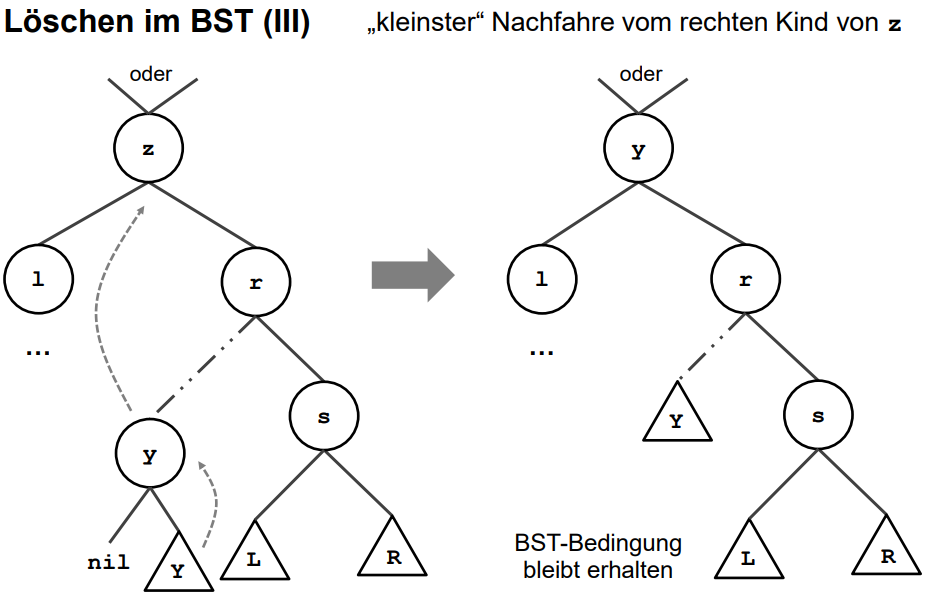
\includegraphics[width=9cm]{pictures/binärerSuchbaumLöschen3.PNG}
    % \caption{Löschen im BST-Fall 3}
\end{figure}
\clearpage
Code:\index{transplant}
%\begin{noindent}
\begin{codeBlock}[autogobble]{title={transplant(T,u,v) // Hängt Teilbaum v an Parent von u}}
    IF u.parent == nil THEN
        T.root = v;
    ELSE
        IF u == u.parent.left THEN
            u.parent.left = v;
        ELSE
            u.parent.right = v;
    IF v != nil THEN
        v.parent = u.parent;
\end{codeBlock}
\begin{codeBlock}[autogobble]{title={delete(T,z)}}
    IF z.left == nil THEN
        transplant(T,z,z.left)
    ELSE
        IF z.right == nil THEN
            transplant(T,z,z,left)
        ELSE
            y = z.right;
            WHILE y.left != nil DO y = y.left;
            IF y.parent != z THEN
                transplant(T,y,y.right)
                y.right = z.right;
                y.right.parent = y;
            transplant(T,z,y)
            y.left = z.left;
            y.left.parent = y;
\end{codeBlock}
%\end{noindent}
Laufzeit = $O(h)$\\
Laufzeit ist damit besser, wenn viele Suchoperationen und $h$ klein relativ zu $n$
\clearpage
\paragraph{Höhe eines BST}
\begin{description}[itemsep=1em]
    \item [Best Case]
          \begin{itemize}
              \item Vollständiger Baum (Alle Blätter gleiche Tiefe)
              \item $h = O(log_2 n)$
              \item Laufzeit = $O(log_2 n)$
          \end{itemize}
    \item [Worst Case]
          \begin{itemize}
              \item Degenerierter Baum (links- bzw. rechtslastiger Baum)
              \item $h = n - 1$
              \item Laufzeit = $\Theta(n)$
          \end{itemize}
    \item [Durchschnittliche Höhe]
          \begin{itemize}
              \item Erwartete Höhe: $\Theta(log_2 n)$
          \end{itemize}
\end{description}
\paragraph{Suchbäume als Suchindex}\index{Suchindex}
\begin{itemize}
    \item Knoten speichert nur Primärschlüssel und Zeiger auf Daten
    \item Zusätzliche Indizes möglich, kosten aber Speicherplatz
\end{itemize}
\begin{figure}[ht]
    \centering
    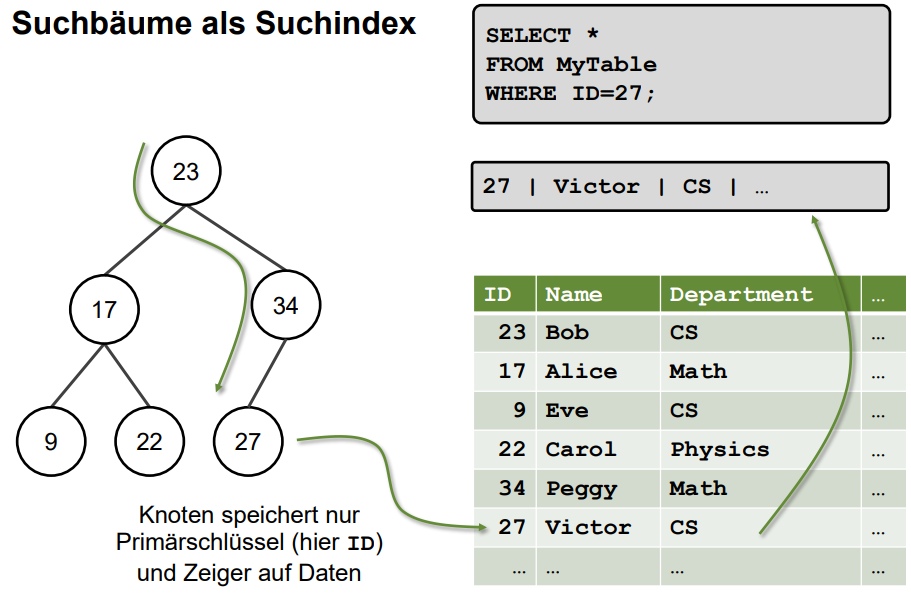
\includegraphics[width=12cm]{pictures/suchbaumSuchindex.PNG}
    \caption{Suchbäume als Suchindex}
\end{figure}
\clearpage
\end{document}
